\documentclass[11pt,fancychapters]{article}
\usepackage[a4paper, total={6in, 8in}]{geometry}
\usepackage{cite}
\usepackage{color}
\usepackage{xcolor}
\usepackage{empheq}
\usepackage{enumitem}
\usepackage{setspace}
\usepackage{hyperref}
\usepackage{minted}
\usepackage{acro}
\usepackage{amsmath}
\usepackage{amsthm}
\usepackage{amssymb}
\usepackage{multirow}
\usepackage{graphicx}
\usepackage{geometry}
\usepackage{subcaption}
\usepackage{cancel}
\usepackage[utf8]{inputenc}
\usepackage[english]{babel}
\usepackage{tcolorbox}
\usepackage{hyperref}
\usepackage{cleveref}
\usepackage{parskip}
\usepackage{tcolorbox}
\usepackage{float}
\usepackage{pgfplots}
 \geometry{
 a4paper,
 total={170mm,257mm},
 left=20mm,
 top=20mm,
 }
\pgfplotsset{width=8cm,compat=1.9}
\newcommand{\dbar}{{d\mkern-7mu\mathchar'26\mkern-2mu}}
\newcommand{\boxedeq}[2]{\begin{empheq}[box={\fboxsep=6pt\fbox}]{align}\label{#1}#2\end{empheq}}
\newcommand{\approptoinn}[2]{\mathrel{\vcenter{
  \offinterlineskip\halign{\hfil$##$\cr
    #1\propto\cr\noalign{\kern2pt}#1\sim\cr\noalign{\kern-2pt}}}}}
\newcommand{\appropto}{\mathpalette\approptoinn\relax}
\renewcommand*{\thesection}{\arabic{section}.}
\def\*#1{\mathbf{#1}}
\def\ab{ab}
\usepackage{tikz}
\usetikzlibrary{calc,trees,positioning,arrows,chains,shapes.geometric,%
    decorations.pathreplacing,decorations.pathmorphing,shapes,%
    matrix,shapes.symbols}
\geometry{top=1.3in,bottom=1.3in}

\begin{document}
\centerline{\huge{SUTD 2021 50.007 Homework 1}}

\begin{table}[ht]
\centering
\footnotesize
 \begin{tabular}{c c} 
James Raphael Tiovalen & 1004555
 \end{tabular}
\end{table}

\section{Classification}

We can plot a visual, graphical representation of the given data points:

\begin{figure}[!h]
\centering
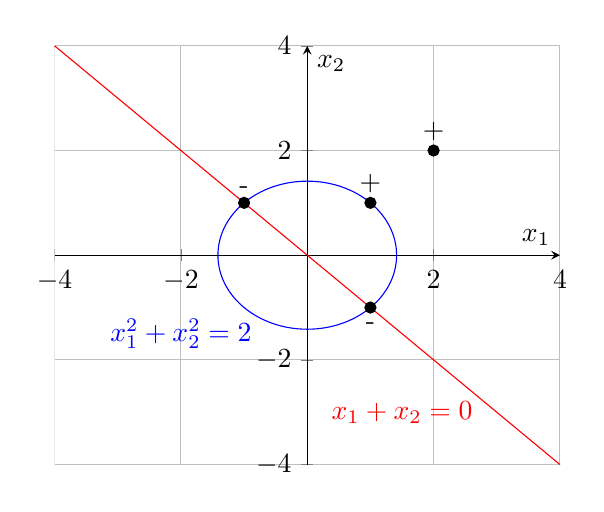
\begin{tikzpicture}
	\begin{axis}[
		axis lines=middle,
		xmin=-4, xmax=4,
		ymin=-4, ymax=4,
		grid=major,
		clip=false,
		xlabel=$x_1$, ylabel=$x_2$,
		]
		\addplot [only marks, mark=*, nodes near coords={\label},
		visualization depends on={value \thisrowno{2} \as \label}] table {
			1 1 +
			2 2 +
		};
		\addplot [only marks, mark=*, nodes near coords={\label},
		visualization depends on={value \thisrowno{2} \as \label}] table {
			-1 1 -
			1 -1 -
		};
		\addplot [color=red, domain=-4:4] {-x}
			node at (axis cs:1.5,-3) {$x_1 + x_2 = 0$};
		\draw [blue, radius=sqrt(2)] (axis cs:0,0) circle
			node at (axis cs:-2,-1.5) {$x_1^2 + x_2^2 = 2$};
	\end{axis}
\end{tikzpicture}
\end{figure}

\begin{enumerate}[label=(\alph*)]

\item Such a classifier does not exist. As demonstrated by the blue-colored circle on the graph above, a minimum radius of $\sqrt{2}$ would be needed to classify the points. However, since the classifier's boundary would intersect two positive points and one negative point (i.e., they lie on the boundary), such a classifier would be insufficient to correctly classify all said data points without any ambiguity. Any classifier of an origin-centered circle with $r < \sqrt{2}$ would classify all the data points with the same label (which is not correct for some of the points), while any classifier of an origin-centered circle with $r > \sqrt{2}$ would classify the two negative data points at $(-1, 1)$ and $(1, -1)$ along with at least the positive data point at $(1, 1)$ under the same label (which is also not correct for some of the points). Hence, no such classifier exists.

\item One and only one possible linear classifier that goes through the origin would be one with a normal vector $\theta = (\theta_1, \theta_2) = (1, 1)$ (or $[\theta_1, \theta_2]^T = [1, 1]^T$). More formally, such a classifier can be defined as

\begin{equation*}
	h(x, \theta) = \text{sign}(x_1 + x_2) = \text{sign}(\theta \cdot x) = \begin{cases}
		+1, \quad &\text{if} \, ~ \theta \cdot x > 0 \\
		-1, \quad &\text{if} \, ~ \theta \cdot x \leq 0 \\
	\end{cases}
\end{equation*}

\end{enumerate}

\end{document}
